\documentclass[10pt]{article}
% Build modes (see Makefile): default = anonymous TMLR submission;
% PREPRINT defined = de-anonymised arXiv preprint.
\ifdefined\PREPRINT
\usepackage[preprint]{tmlr}
\else
\usepackage{tmlr}
\fi

%%%%% NEW MATH DEFINITIONS %%%%%

\usepackage{amsmath,amsfonts,bm}

% Mark sections of captions for referring to divisions of figures
\newcommand{\figleft}{{\em (Left)}}
\newcommand{\figcenter}{{\em (Center)}}
\newcommand{\figright}{{\em (Right)}}
\newcommand{\figtop}{{\em (Top)}}
\newcommand{\figbottom}{{\em (Bottom)}}
\newcommand{\captiona}{{\em (a)}}
\newcommand{\captionb}{{\em (b)}}
\newcommand{\captionc}{{\em (c)}}
\newcommand{\captiond}{{\em (d)}}

% Highlight a newly defined term
\newcommand{\newterm}[1]{{\bf #1}}


% Figure reference, lower-case.
\def\figref#1{figure~\ref{#1}}
% Figure reference, capital. For start of sentence
\def\Figref#1{Figure~\ref{#1}}
\def\twofigref#1#2{figures \ref{#1} and \ref{#2}}
\def\quadfigref#1#2#3#4{figures \ref{#1}, \ref{#2}, \ref{#3} and \ref{#4}}
% Section reference, lower-case.
\def\secref#1{section~\ref{#1}}
% Section reference, capital.
\def\Secref#1{Section~\ref{#1}}
% Reference to two sections.
\def\twosecrefs#1#2{sections \ref{#1} and \ref{#2}}
% Reference to three sections.
\def\secrefs#1#2#3{sections \ref{#1}, \ref{#2} and \ref{#3}}
% Reference to an equation, lower-case.
\def\eqref#1{equation~\ref{#1}}
% Reference to an equation, upper case
\def\Eqref#1{Equation~\ref{#1}}
% A raw reference to an equation---avoid using if possible
\def\plaineqref#1{\ref{#1}}
% Reference to a chapter, lower-case.
\def\chapref#1{chapter~\ref{#1}}
% Reference to an equation, upper case.
\def\Chapref#1{Chapter~\ref{#1}}
% Reference to a range of chapters
\def\rangechapref#1#2{chapters\ref{#1}--\ref{#2}}
% Reference to an algorithm, lower-case.
\def\algref#1{algorithm~\ref{#1}}
% Reference to an algorithm, upper case.
\def\Algref#1{Algorithm~\ref{#1}}
\def\twoalgref#1#2{algorithms \ref{#1} and \ref{#2}}
\def\Twoalgref#1#2{Algorithms \ref{#1} and \ref{#2}}
% Reference to a part, lower case
\def\partref#1{part~\ref{#1}}
% Reference to a part, upper case
\def\Partref#1{Part~\ref{#1}}
\def\twopartref#1#2{parts \ref{#1} and \ref{#2}}

\def\ceil#1{\lceil #1 \rceil}
\def\floor#1{\lfloor #1 \rfloor}
\def\1{\bm{1}}
\newcommand{\train}{\mathcal{D}}
\newcommand{\valid}{\mathcal{D_{\mathrm{valid}}}}
\newcommand{\test}{\mathcal{D_{\mathrm{test}}}}

\def\eps{{\epsilon}}


% Random variables
\def\reta{{\textnormal{$\eta$}}}
\def\ra{{\textnormal{a}}}
\def\rb{{\textnormal{b}}}
\def\rc{{\textnormal{c}}}
\def\rd{{\textnormal{d}}}
\def\re{{\textnormal{e}}}
\def\rf{{\textnormal{f}}}
\def\rg{{\textnormal{g}}}
\def\rh{{\textnormal{h}}}
\def\ri{{\textnormal{i}}}
\def\rj{{\textnormal{j}}}
\def\rk{{\textnormal{k}}}
\def\rl{{\textnormal{l}}}
% rm is already a command, just don't name any random variables m
\def\rn{{\textnormal{n}}}
\def\ro{{\textnormal{o}}}
\def\rp{{\textnormal{p}}}
\def\rq{{\textnormal{q}}}
\def\rr{{\textnormal{r}}}
\def\rs{{\textnormal{s}}}
\def\rt{{\textnormal{t}}}
\def\ru{{\textnormal{u}}}
\def\rv{{\textnormal{v}}}
\def\rw{{\textnormal{w}}}
\def\rx{{\textnormal{x}}}
\def\ry{{\textnormal{y}}}
\def\rz{{\textnormal{z}}}

% Random vectors
\def\rvepsilon{{\mathbf{\epsilon}}}
\def\rvtheta{{\mathbf{\theta}}}
\def\rva{{\mathbf{a}}}
\def\rvb{{\mathbf{b}}}
\def\rvc{{\mathbf{c}}}
\def\rvd{{\mathbf{d}}}
\def\rve{{\mathbf{e}}}
\def\rvf{{\mathbf{f}}}
\def\rvg{{\mathbf{g}}}
\def\rvh{{\mathbf{h}}}
\def\rvu{{\mathbf{i}}}
\def\rvj{{\mathbf{j}}}
\def\rvk{{\mathbf{k}}}
\def\rvl{{\mathbf{l}}}
\def\rvm{{\mathbf{m}}}
\def\rvn{{\mathbf{n}}}
\def\rvo{{\mathbf{o}}}
\def\rvp{{\mathbf{p}}}
\def\rvq{{\mathbf{q}}}
\def\rvr{{\mathbf{r}}}
\def\rvs{{\mathbf{s}}}
\def\rvt{{\mathbf{t}}}
\def\rvu{{\mathbf{u}}}
\def\rvv{{\mathbf{v}}}
\def\rvw{{\mathbf{w}}}
\def\rvx{{\mathbf{x}}}
\def\rvy{{\mathbf{y}}}
\def\rvz{{\mathbf{z}}}

% Elements of random vectors
\def\erva{{\textnormal{a}}}
\def\ervb{{\textnormal{b}}}
\def\ervc{{\textnormal{c}}}
\def\ervd{{\textnormal{d}}}
\def\erve{{\textnormal{e}}}
\def\ervf{{\textnormal{f}}}
\def\ervg{{\textnormal{g}}}
\def\ervh{{\textnormal{h}}}
\def\ervi{{\textnormal{i}}}
\def\ervj{{\textnormal{j}}}
\def\ervk{{\textnormal{k}}}
\def\ervl{{\textnormal{l}}}
\def\ervm{{\textnormal{m}}}
\def\ervn{{\textnormal{n}}}
\def\ervo{{\textnormal{o}}}
\def\ervp{{\textnormal{p}}}
\def\ervq{{\textnormal{q}}}
\def\ervr{{\textnormal{r}}}
\def\ervs{{\textnormal{s}}}
\def\ervt{{\textnormal{t}}}
\def\ervu{{\textnormal{u}}}
\def\ervv{{\textnormal{v}}}
\def\ervw{{\textnormal{w}}}
\def\ervx{{\textnormal{x}}}
\def\ervy{{\textnormal{y}}}
\def\ervz{{\textnormal{z}}}

% Random matrices
\def\rmA{{\mathbf{A}}}
\def\rmB{{\mathbf{B}}}
\def\rmC{{\mathbf{C}}}
\def\rmD{{\mathbf{D}}}
\def\rmE{{\mathbf{E}}}
\def\rmF{{\mathbf{F}}}
\def\rmG{{\mathbf{G}}}
\def\rmH{{\mathbf{H}}}
\def\rmI{{\mathbf{I}}}
\def\rmJ{{\mathbf{J}}}
\def\rmK{{\mathbf{K}}}
\def\rmL{{\mathbf{L}}}
\def\rmM{{\mathbf{M}}}
\def\rmN{{\mathbf{N}}}
\def\rmO{{\mathbf{O}}}
\def\rmP{{\mathbf{P}}}
\def\rmQ{{\mathbf{Q}}}
\def\rmR{{\mathbf{R}}}
\def\rmS{{\mathbf{S}}}
\def\rmT{{\mathbf{T}}}
\def\rmU{{\mathbf{U}}}
\def\rmV{{\mathbf{V}}}
\def\rmW{{\mathbf{W}}}
\def\rmX{{\mathbf{X}}}
\def\rmY{{\mathbf{Y}}}
\def\rmZ{{\mathbf{Z}}}

% Elements of random matrices
\def\ermA{{\textnormal{A}}}
\def\ermB{{\textnormal{B}}}
\def\ermC{{\textnormal{C}}}
\def\ermD{{\textnormal{D}}}
\def\ermE{{\textnormal{E}}}
\def\ermF{{\textnormal{F}}}
\def\ermG{{\textnormal{G}}}
\def\ermH{{\textnormal{H}}}
\def\ermI{{\textnormal{I}}}
\def\ermJ{{\textnormal{J}}}
\def\ermK{{\textnormal{K}}}
\def\ermL{{\textnormal{L}}}
\def\ermM{{\textnormal{M}}}
\def\ermN{{\textnormal{N}}}
\def\ermO{{\textnormal{O}}}
\def\ermP{{\textnormal{P}}}
\def\ermQ{{\textnormal{Q}}}
\def\ermR{{\textnormal{R}}}
\def\ermS{{\textnormal{S}}}
\def\ermT{{\textnormal{T}}}
\def\ermU{{\textnormal{U}}}
\def\ermV{{\textnormal{V}}}
\def\ermW{{\textnormal{W}}}
\def\ermX{{\textnormal{X}}}
\def\ermY{{\textnormal{Y}}}
\def\ermZ{{\textnormal{Z}}}

% Vectors
\def\vzero{{\bm{0}}}
\def\vone{{\bm{1}}}
\def\vmu{{\bm{\mu}}}
\def\vtheta{{\bm{\theta}}}
\def\va{{\bm{a}}}
\def\vb{{\bm{b}}}
\def\vc{{\bm{c}}}
\def\vd{{\bm{d}}}
\def\ve{{\bm{e}}}
\def\vf{{\bm{f}}}
\def\vg{{\bm{g}}}
\def\vh{{\bm{h}}}
\def\vi{{\bm{i}}}
\def\vj{{\bm{j}}}
\def\vk{{\bm{k}}}
\def\vl{{\bm{l}}}
\def\vm{{\bm{m}}}
\def\vn{{\bm{n}}}
\def\vo{{\bm{o}}}
\def\vp{{\bm{p}}}
\def\vq{{\bm{q}}}
\def\vr{{\bm{r}}}
\def\vs{{\bm{s}}}
\def\vt{{\bm{t}}}
\def\vu{{\bm{u}}}
\def\vv{{\bm{v}}}
\def\vw{{\bm{w}}}
\def\vx{{\bm{x}}}
\def\vy{{\bm{y}}}
\def\vz{{\bm{z}}}

% Elements of vectors
\def\evalpha{{\alpha}}
\def\evbeta{{\beta}}
\def\evepsilon{{\epsilon}}
\def\evlambda{{\lambda}}
\def\evomega{{\omega}}
\def\evmu{{\mu}}
\def\evpsi{{\psi}}
\def\evsigma{{\sigma}}
\def\evtheta{{\theta}}
\def\eva{{a}}
\def\evb{{b}}
\def\evc{{c}}
\def\evd{{d}}
\def\eve{{e}}
\def\evf{{f}}
\def\evg{{g}}
\def\evh{{h}}
\def\evi{{i}}
\def\evj{{j}}
\def\evk{{k}}
\def\evl{{l}}
\def\evm{{m}}
\def\evn{{n}}
\def\evo{{o}}
\def\evp{{p}}
\def\evq{{q}}
\def\evr{{r}}
\def\evs{{s}}
\def\evt{{t}}
\def\evu{{u}}
\def\evv{{v}}
\def\evw{{w}}
\def\evx{{x}}
\def\evy{{y}}
\def\evz{{z}}

% Matrix
\def\mA{{\bm{A}}}
\def\mB{{\bm{B}}}
\def\mC{{\bm{C}}}
\def\mD{{\bm{D}}}
\def\mE{{\bm{E}}}
\def\mF{{\bm{F}}}
\def\mG{{\bm{G}}}
\def\mH{{\bm{H}}}
\def\mI{{\bm{I}}}
\def\mJ{{\bm{J}}}
\def\mK{{\bm{K}}}
\def\mL{{\bm{L}}}
\def\mM{{\bm{M}}}
\def\mN{{\bm{N}}}
\def\mO{{\bm{O}}}
\def\mP{{\bm{P}}}
\def\mQ{{\bm{Q}}}
\def\mR{{\bm{R}}}
\def\mS{{\bm{S}}}
\def\mT{{\bm{T}}}
\def\mU{{\bm{U}}}
\def\mV{{\bm{V}}}
\def\mW{{\bm{W}}}
\def\mX{{\bm{X}}}
\def\mY{{\bm{Y}}}
\def\mZ{{\bm{Z}}}
\def\mBeta{{\bm{\beta}}}
\def\mPhi{{\bm{\Phi}}}
\def\mLambda{{\bm{\Lambda}}}
\def\mSigma{{\bm{\Sigma}}}

% Tensor
\DeclareMathAlphabet{\mathsfit}{\encodingdefault}{\sfdefault}{m}{sl}
\SetMathAlphabet{\mathsfit}{bold}{\encodingdefault}{\sfdefault}{bx}{n}
\newcommand{\tens}[1]{\bm{\mathsfit{#1}}}
\def\tA{{\tens{A}}}
\def\tB{{\tens{B}}}
\def\tC{{\tens{C}}}
\def\tD{{\tens{D}}}
\def\tE{{\tens{E}}}
\def\tF{{\tens{F}}}
\def\tG{{\tens{G}}}
\def\tH{{\tens{H}}}
\def\tI{{\tens{I}}}
\def\tJ{{\tens{J}}}
\def\tK{{\tens{K}}}
\def\tL{{\tens{L}}}
\def\tM{{\tens{M}}}
\def\tN{{\tens{N}}}
\def\tO{{\tens{O}}}
\def\tP{{\tens{P}}}
\def\tQ{{\tens{Q}}}
\def\tR{{\tens{R}}}
\def\tS{{\tens{S}}}
\def\tT{{\tens{T}}}
\def\tU{{\tens{U}}}
\def\tV{{\tens{V}}}
\def\tW{{\tens{W}}}
\def\tX{{\tens{X}}}
\def\tY{{\tens{Y}}}
\def\tZ{{\tens{Z}}}


% Graph
\def\gA{{\mathcal{A}}}
\def\gB{{\mathcal{B}}}
\def\gC{{\mathcal{C}}}
\def\gD{{\mathcal{D}}}
\def\gE{{\mathcal{E}}}
\def\gF{{\mathcal{F}}}
\def\gG{{\mathcal{G}}}
\def\gH{{\mathcal{H}}}
\def\gI{{\mathcal{I}}}
\def\gJ{{\mathcal{J}}}
\def\gK{{\mathcal{K}}}
\def\gL{{\mathcal{L}}}
\def\gM{{\mathcal{M}}}
\def\gN{{\mathcal{N}}}
\def\gO{{\mathcal{O}}}
\def\gP{{\mathcal{P}}}
\def\gQ{{\mathcal{Q}}}
\def\gR{{\mathcal{R}}}
\def\gS{{\mathcal{S}}}
\def\gT{{\mathcal{T}}}
\def\gU{{\mathcal{U}}}
\def\gV{{\mathcal{V}}}
\def\gW{{\mathcal{W}}}
\def\gX{{\mathcal{X}}}
\def\gY{{\mathcal{Y}}}
\def\gZ{{\mathcal{Z}}}

% Sets
\def\sA{{\mathbb{A}}}
\def\sB{{\mathbb{B}}}
\def\sC{{\mathbb{C}}}
\def\sD{{\mathbb{D}}}
% Don't use a set called E, because this would be the same as our symbol
% for expectation.
\def\sF{{\mathbb{F}}}
\def\sG{{\mathbb{G}}}
\def\sH{{\mathbb{H}}}
\def\sI{{\mathbb{I}}}
\def\sJ{{\mathbb{J}}}
\def\sK{{\mathbb{K}}}
\def\sL{{\mathbb{L}}}
\def\sM{{\mathbb{M}}}
\def\sN{{\mathbb{N}}}
\def\sO{{\mathbb{O}}}
\def\sP{{\mathbb{P}}}
\def\sQ{{\mathbb{Q}}}
\def\sR{{\mathbb{R}}}
\def\sS{{\mathbb{S}}}
\def\sT{{\mathbb{T}}}
\def\sU{{\mathbb{U}}}
\def\sV{{\mathbb{V}}}
\def\sW{{\mathbb{W}}}
\def\sX{{\mathbb{X}}}
\def\sY{{\mathbb{Y}}}
\def\sZ{{\mathbb{Z}}}

% Entries of a matrix
\def\emLambda{{\Lambda}}
\def\emA{{A}}
\def\emB{{B}}
\def\emC{{C}}
\def\emD{{D}}
\def\emE{{E}}
\def\emF{{F}}
\def\emG{{G}}
\def\emH{{H}}
\def\emI{{I}}
\def\emJ{{J}}
\def\emK{{K}}
\def\emL{{L}}
\def\emM{{M}}
\def\emN{{N}}
\def\emO{{O}}
\def\emP{{P}}
\def\emQ{{Q}}
\def\emR{{R}}
\def\emS{{S}}
\def\emT{{T}}
\def\emU{{U}}
\def\emV{{V}}
\def\emW{{W}}
\def\emX{{X}}
\def\emY{{Y}}
\def\emZ{{Z}}
\def\emSigma{{\Sigma}}

% entries of a tensor
% Same font as tensor, without \bm wrapper
\newcommand{\etens}[1]{\mathsfit{#1}}
\def\etLambda{{\etens{\Lambda}}}
\def\etA{{\etens{A}}}
\def\etB{{\etens{B}}}
\def\etC{{\etens{C}}}
\def\etD{{\etens{D}}}
\def\etE{{\etens{E}}}
\def\etF{{\etens{F}}}
\def\etG{{\etens{G}}}
\def\etH{{\etens{H}}}
\def\etI{{\etens{I}}}
\def\etJ{{\etens{J}}}
\def\etK{{\etens{K}}}
\def\etL{{\etens{L}}}
\def\etM{{\etens{M}}}
\def\etN{{\etens{N}}}
\def\etO{{\etens{O}}}
\def\etP{{\etens{P}}}
\def\etQ{{\etens{Q}}}
\def\etR{{\etens{R}}}
\def\etS{{\etens{S}}}
\def\etT{{\etens{T}}}
\def\etU{{\etens{U}}}
\def\etV{{\etens{V}}}
\def\etW{{\etens{W}}}
\def\etX{{\etens{X}}}
\def\etY{{\etens{Y}}}
\def\etZ{{\etens{Z}}}

% The true underlying data generating distribution
\newcommand{\pdata}{p_{\rm{data}}}
% The empirical distribution defined by the training set
\newcommand{\ptrain}{\hat{p}_{\rm{data}}}
\newcommand{\Ptrain}{\hat{P}_{\rm{data}}}
% The model distribution
\newcommand{\pmodel}{p_{\rm{model}}}
\newcommand{\Pmodel}{P_{\rm{model}}}
\newcommand{\ptildemodel}{\tilde{p}_{\rm{model}}}
% Stochastic autoencoder distributions
\newcommand{\pencode}{p_{\rm{encoder}}}
\newcommand{\pdecode}{p_{\rm{decoder}}}
\newcommand{\precons}{p_{\rm{reconstruct}}}

\newcommand{\laplace}{\mathrm{Laplace}} % Laplace distribution

\newcommand{\E}{\mathbb{E}}
\newcommand{\Ls}{\mathcal{L}}
\newcommand{\R}{\mathbb{R}}
\newcommand{\emp}{\tilde{p}}
\newcommand{\lr}{\alpha}
\newcommand{\reg}{\lambda}
\newcommand{\rect}{\mathrm{rectifier}}
\newcommand{\softmax}{\mathrm{softmax}}
\newcommand{\sigmoid}{\sigma}
\newcommand{\softplus}{\zeta}
\newcommand{\KL}{D_{\mathrm{KL}}}
\newcommand{\Var}{\mathrm{Var}}
\newcommand{\standarderror}{\mathrm{SE}}
\newcommand{\Cov}{\mathrm{Cov}}
% Wolfram Mathworld says $L^2$ is for function spaces and $\ell^2$ is for vectors
% But then they seem to use $L^2$ for vectors throughout the site, and so does
% wikipedia.
\newcommand{\normlzero}{L^0}
\newcommand{\normlone}{L^1}
\newcommand{\normltwo}{L^2}
\newcommand{\normlp}{L^p}
\newcommand{\normmax}{L^\infty}

\newcommand{\parents}{Pa} % See usage in notation.tex. Chosen to match Daphne's book.

\DeclareMathOperator*{\argmax}{arg\,max}
\DeclareMathOperator*{\argmin}{arg\,min}

\DeclareMathOperator{\sign}{sign}
\DeclareMathOperator{\Tr}{Tr}
\let\ab\allowbreak

\usepackage{hyperref}
\usepackage{url}
\usepackage{booktabs}
\usepackage{graphicx}
\usepackage{amsmath,amssymb}
\usepackage{float}

\title{Speaker Identity Is Split Across Conditioning Sites:\\
Prompt and Embedding Pathways in Zero-Shot Voice Cloning}

\author{\name Callum Macpherson \email REPLACE\_WITH\_EMAIL \\
      \addr Independent researcher}

\def\month{MM}
\def\year{YYYY}
\def\openreview{\url{https://openreview.net/forum?id=XXXX}}

\begin{document}
\maketitle

\begin{abstract}
Zero-shot text-to-speech (TTS) systems clone a voice from a few seconds of reference audio, and most of them condition on that reference through two routes at once: an in-context acoustic \emph{prompt} and a global speaker \emph{embedding}. Systems differ in where the embedding enters: some inject it into the autoregressive language model (LM) that generates speech tokens, others only into the acoustic decoder that renders them. We ask what each route and each site carries. First, across six open-weight systems and two test sets (25{,}509 synthesised utterances), we remove the prompt while keeping the embedding and find that identity survives best when the embedding also conditions the LM. Second, in CosyVoice, which injects the same embedding at both sites, a within-model $2{\times}2{\times}2$ factorial (6{,}480 utterances) switches the prompt, the LM embedding and the decoder embedding on and off independently. Without the prompt, the two sites contribute additively to speaker similarity (about 0.10 and 0.19 SIM-o); with the prompt, the LM embedding becomes redundant while the decoder embedding does not, so the prompt can stand in for one site but not the other. Third, prompts carry their recording conditions into the output, and the predicted-naturalness gain from dropping them partly reflects a metric that also rewards generic voices. We release code, job lists and scores.
\end{abstract}

%======================================================================
\section{Introduction}
\label{sec:intro}
%======================================================================

Zero-shot TTS has moved from research curiosity to deployed technology: systems such as VALL-E~\citep{valle}, Seed-TTS~\citep{seedtts}, Voicebox~\citep{voicebox}, CosyVoice~\citep{cosyvoice,cosyvoice2,cosyvoice3} and Qwen3-TTS~\citep{qwen3tts} reproduce a speaker from seconds of audio.
Most of these systems are two-stage generators: an autoregressive language model produces discrete speech tokens, and an acoustic decoder (a flow-matching model, a diffusion model or a vocoder) turns them into a waveform.
They condition on the target speaker through two routes.
The \emph{acoustic prompt} places the reference's speech tokens or features in context, so the LM continues them and the decoder can copy fine acoustic detail.
The \emph{speaker embedding} summarises the reference as one vector from a speaker-verification encoder.
Systems also differ in where the embedding enters, which we call its \emph{site}: Qwen3-TTS feeds it to the LM, CosyVoice to both the LM and the decoder, while CosyVoice~2/3 and XTTS-v2 feed it only to the decoder.

These design choices are made, and changed, without measurement.
CosyVoice~2 removed the embedding from its LM ``to avoid information leaking''~\citep{cosyvoice2}, and later work describes this as an interface redesign~\citep{chen2026bottleneck}, but what the LM-site embedding contributed was never quantified.
The question matters beyond architecture.
Prompts are known to import their acoustic environment~\citep{lu2025noise,wang2024noise}; prompt-free conditioning is attractive for streaming, cross-lingual and privacy-preserving use; and if an embedding alone carries identity, speaker embeddings are identity-bearing data that warrant protection.

We treat the two routes and the embedding sites as experimental variables and intervene on them directly.
Our contributions are:
\begin{enumerate}
  \item \textbf{A matched cross-system intervention.} In six open-weight systems we remove all prompt-level conditioning while keeping the speaker embedding, on clean (LibriTTS-R) and noisy (Seed-TTS-eval) prompts, scored with the Seed-TTS-eval protocol and speaker-level statistics (Section~\ref{sec:cross}).
  \item \textbf{A within-model causal factorial.} In CosyVoice, which injects one embedding at two sites, we cross prompt $\times$ LM embedding $\times$ decoder embedding. Identity is split additively across the sites, and the prompt substitutes for the embedding at the LM but not at the decoder (Section~\ref{sec:factorial}).
  \item \textbf{What the prompt carries besides identity.} Outputs reproduce the specific prompt recording, so dropping the prompt helps most for noisy prompts; we also show that the naturalness predictor rewards losing identity, which qualifies naturalness gains reported for prompt-free conditioning (Section~\ref{sec:recording}).
  \item \textbf{Reference count.} Three references improve similarity slightly but reliably in either route without changing naturalness, while a prompt-only system degrades (Section~\ref{sec:refcount}).
\end{enumerate}

%======================================================================
\section{Related Work}
\label{sec:related}
%======================================================================

\paragraph{Speaker conditioning in zero-shot TTS.}
Codec language models such as VALL-E~\citep{valle} rely on an acoustic prompt only, as does the flow-matching F5-TTS~\citep{f5tts}; StyleTTS~2~\citep{styletts2} relies on a style embedding.
Multi-speaker systems such as YourTTS~\citep{yourtts} condition on a speaker encoder, and comparisons of encoders vary the embedding rather than the route.
CosyVoice~\citep{cosyvoice} conditions both its LM and its flow decoder on an x-vector; CosyVoice~2 and~3~\citep{cosyvoice2,cosyvoice3} keep it only in the flow; XTTS~\citep{xtts} uses GPT conditioning latents for the LM and a speaker embedding for the decoder; Qwen3-TTS~\citep{qwen3tts} injects the embedding as an LM input in both its in-context and its x-vector-only modes.
To our knowledge no prior work measures what each route or site contributes.

\paragraph{Prompts, references and robustness.}
Longer or multiple prompts help when a model is trained for them~\citep{megatts2,lei2023multiscale,pfluxtts}.
Prompt noise propagates into the output of LLM- and flow-based TTS~\citep{lu2025noise,wang2024noise}, and RVCBench evaluates 18 cloning systems under noisy references and other shifts~\citep{rvcbench}.
These works vary the reference; we keep it fixed and vary which conditioning route and site receive it.

\paragraph{Evaluation methodology.}
We follow the Seed-TTS-eval protocol~\citep{seedtts} and recent guidance on reporting~\citep{kirkland2023mos,wester2015listeners}, with speakers as the unit of analysis.

%======================================================================
\section{Method}
\label{sec:method}
%======================================================================

\subsection{Systems and conditioning sites}

Table~\ref{tab:systems} lists the systems and where their embedding enters, verified in each released inference code base.
In the \emph{full} condition a system receives its usual prompt and embedding from one reference.
In the \emph{x-vector only} condition we remove all prompt-level conditioning and keep the embedding: Qwen3-TTS's native \texttt{x\_vector\_only} mode; for CosyVoice and CosyVoice~3, the prompt speech tokens and features are removed from both the LM and the flow decoder (CosyVoice~3 keeps its required system-prompt text prefix); for XTTS-v2, whose LM conditioning \emph{is} its prompt latents, these are replaced by a fixed mean over two held-out speakers; for Chatterbox, the T3 speech-prompt tokens are removed.
Because the interventions are system-specific, the cross-system study compares patterns, and the causal claim rests on the within-model factorial.
F5-TTS, which has no embedding route, is a prompt-only control for the reference-count study.

\begin{table}[t]
\centering
\caption{Systems, where their speaker embedding enters, and what the x-vector-only condition removes.}
\label{tab:systems}
\small
\resizebox{\textwidth}{!}{%
\begin{tabular}{llll}
\toprule
\textbf{System} & \textbf{Licence} & \textbf{Embedding enters} & \textbf{Prompt removed} \\
\midrule
Qwen3-TTS 0.6B, 1.7B~\citep{qwen3tts} & Apache-2.0 & LM input & ICL codec prompt \\
CosyVoice-300M~\citep{cosyvoice} & Apache-2.0 & LM and flow decoder & LM and flow prompt \\
CosyVoice~3 0.5B~\citep{cosyvoice3} & Apache-2.0 & flow decoder only & LM and flow prompt \\
XTTS-v2~\citep{xtts} & CPML (non-commercial) & vocoder decoder only & GPT conditioning latents \\
Chatterbox~\citep{chatterbox} & MIT & LM (T3) & T3 speech prompt \\
F5-TTS v1~\citep{f5tts} & CC-BY-NC-4.0 & none (control) & --- \\
\bottomrule
\end{tabular}%
}
\end{table}

\subsection{Within-model embedding-site factorial}

CosyVoice-300M passes the same CAM++ embedding to its LM (\texttt{llm\_embedding}) and its flow decoder (\texttt{flow\_embedding}); both modules L2-normalise it before an affine projection.
We cross three switches: prompt (present or removed, as above), LM embedding (kept or zeroed) and decoder embedding (kept or zeroed).
Zeroing removes the speaker signal and leaves the projection's bias, the same ablation used in the original CosyVoice code paths.
Everything else (text, reference, seed, decoding) is identical across the eight cells.

\subsection{Data and design}

\textbf{LibriTTS-R}~\citep{libritts_r,libritts}: 34 sex-balanced \texttt{test-clean} speakers, 5 target sentences each, one fixed 6\,s reference per speaker, seeds 42--44.
\textbf{Seed-TTS-eval test-en}~\citep{seedtts}: 1{,}088 items, each with its own Common Voice prompt (666 distinct prompt speakers), seed 42; these prompts are noisier and more varied than audiobook speech.
The site factorial uses all LibriTTS-R cells and a fixed random 300-item Seed-TTS-eval subset (268 prompt speakers).
The reference-count study draws $n \in \{1,3\}$ references of 3--9.5\,s per LibriTTS-R speaker (by duration or at random), either concatenated in the prompt or averaged as embeddings.
Prompts are built at 24\,kHz.
In total we synthesised 31{,}989 utterances; 25 of 25{,}534 planned pathway utterances failed (all Chatterbox, Table~\ref{tab:failures}) and none in the factorial.

\subsection{Metrics and statistics}

\textbf{SIM-o} is the cosine similarity of WavLM-large speaker-verification embeddings (the Seed-TTS-eval checkpoint) between the output and a \emph{held-out} recording of the speaker: the ground-truth target recording for Seed-TTS-eval, and for LibriTTS-R a recording longer than 9.5\,s never used as prompt or target.
\textbf{SIM-p} is the same similarity to the prompt itself; SIM-p minus SIM-o measures how much the output resembles the specific prompt recording beyond the speaker.
\textbf{WER} uses Whisper-large-v3~\citep{whisper} with the Seed-TTS-eval normalisation.
\textbf{Naturalness} is predicted with UTMOS~\citep{utmos}; on the earlier confirmatory audio, UTMOSv2~\citep{utmosv2} gives the same direction for every system, and Parakeet-TDT~\citep{parakeet} WER correlates with Whisper WER at Spearman $\rho{=}0.78$.
Targets and seeds are repeated measures, so speakers are the unit of analysis: we average within speaker and condition, test paired speaker-level differences with Wilcoxon signed-rank tests with Holm correction over all contrasts in a family, and report speaker-level bootstrap 95\% CIs (2{,}000 resamples).

%======================================================================
\section{Results}
\label{sec:results}
%======================================================================

\begin{figure}[t]
  \centering
  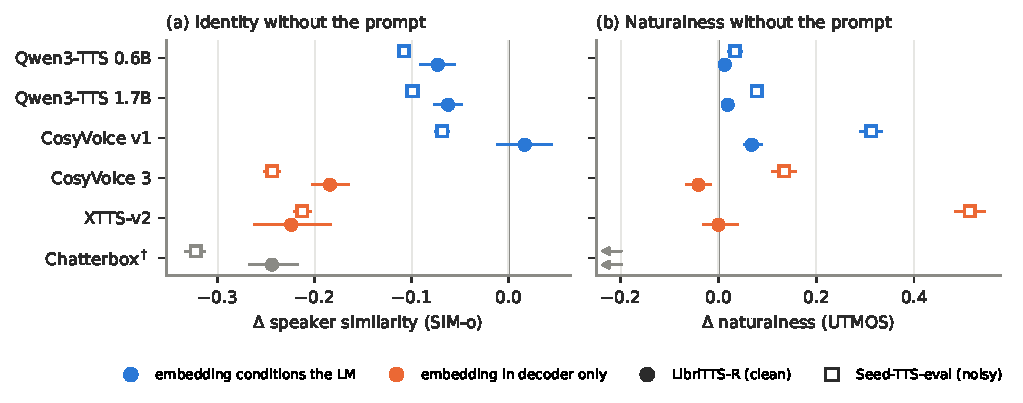
\includegraphics[width=\textwidth]{figures/pathway_headline}
  \caption{Removing prompt-level conditioning across systems (x-vector only minus full; speaker-level means, 95\% bootstrap CIs). (a)~Systems whose LM also receives the embedding (blue) keep more identity than decoder-only systems (orange). (b)~Predicted naturalness rises most on noisy Seed-TTS-eval prompts (squares). $^\dagger$Chatterbox stops producing intelligible speech without its prompt (UTMOS $-1.8$, off-scale).}
  \label{fig:cross}
\end{figure}

\subsection{Across systems, an LM site helps identity survive}
\label{sec:cross}

Figure~\ref{fig:cross}a and Table~\ref{tab:contrasts} (Appendix) show the change in SIM-o when the prompt is removed.
In the two systems whose LM receives the embedding and that still synthesise intelligible speech, identity largely survives: Qwen3-TTS loses 0.062--0.073 on LibriTTS-R and 0.099--0.108 on Seed-TTS-eval at both sizes, and CosyVoice loses nothing on LibriTTS-R ($+0.017$, n.s.) and 0.068 on Seed-TTS-eval.
In the two decoder-only systems the losses are two to three times larger: CosyVoice~3 loses 0.184 and 0.244, and XTTS-v2 0.224 and 0.213 (all $p_\text{Holm}{<}0.001$).
CosyVoice and its successor CosyVoice~3 share a lineage and front end and differ in whether the LM sees the embedding; the successor loses 0.18 where its predecessor loses nothing on LibriTTS-R.
Chatterbox is the exception: its LM receives an embedding, yet without its speech prompt it produces unintelligible speech (WER 96--98\%), so the embedding alone is outside its operating regime.
With the prompt, WER is 1.7--5.9\% for all systems, and removing the prompt leaves WER unchanged except for Chatterbox.
Because these systems differ in data, scale, tokenisers and decoders, we next test the role of each site within one model.

\subsection{Within CosyVoice, identity is split across sites}
\label{sec:factorial}

\begin{figure}[t]
  \centering
  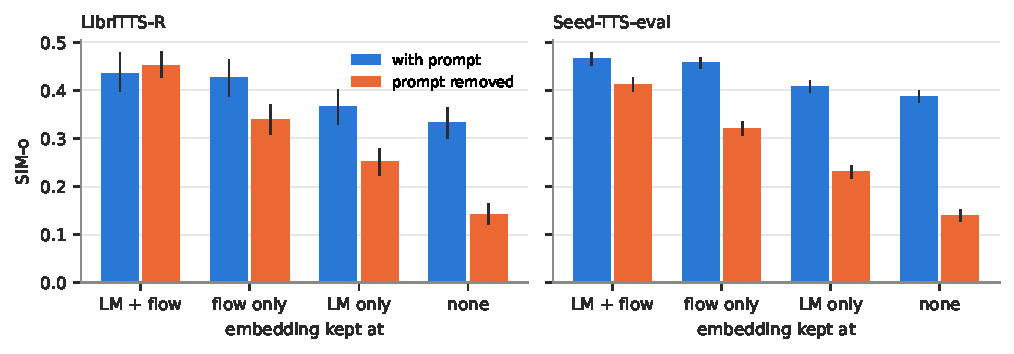
\includegraphics[width=\textwidth]{figures/sites_factorial}
  \caption{CosyVoice embedding-site factorial. SIM-o (speaker-level means, 95\% bootstrap CIs) for each combination of prompt (blue: kept, orange: removed) and embedding sites. Without the prompt, each site carries part of the identity and the losses add; with the prompt, removing the LM embedding has no effect.}
  \label{fig:factorial}
\end{figure}

\begin{table}[t]
\centering
\caption{Embedding-site effects in CosyVoice: change in SIM-o from the all-sites-on cell within each prompt condition (speaker-level, 95\% bootstrap CI, Wilcoxon $p$).}
\label{tab:factorial}
\small
\begin{tabular}{llcc}
\toprule
\textbf{Prompt} & \textbf{Embedding removed at} & \textbf{LibriTTS-R} (34 spk) & \textbf{Seed-TTS-eval} (268 spk) \\
\midrule
removed & LM & $-0.113$ \scriptsize{[$-0.140$, $-0.084$], $p{<}10^{-8}$} & $-0.092$ \scriptsize{[$-0.109$, $-0.075$], $p{<}10^{-18}$} \\
removed & decoder & $-0.201$ \scriptsize{[$-0.225$, $-0.176$], $p{<}10^{-9}$} & $-0.181$ \scriptsize{[$-0.192$, $-0.170$], $p{<}10^{-44}$} \\
removed & both & $-0.310$ \scriptsize{[$-0.339$, $-0.282$], $p{<}10^{-9}$} & $-0.272$ \scriptsize{[$-0.288$, $-0.256$], $p{<}10^{-44}$} \\
\midrule
kept & LM & $-0.010$ \scriptsize{[$-0.023$, $+0.003$], $p{=}0.2$} & $-0.008$ \scriptsize{[$-0.018$, $+0.002$], $p{=}0.07$} \\
kept & decoder & $-0.070$ \scriptsize{[$-0.083$, $-0.058$], $p{<}10^{-9}$} & $-0.057$ \scriptsize{[$-0.064$, $-0.051$], $p{<}10^{-37}$} \\
kept & both & $-0.102$ \scriptsize{[$-0.123$, $-0.084$], $p{<}10^{-9}$} & $-0.078$ \scriptsize{[$-0.090$, $-0.066$], $p{<}10^{-27}$} \\
\bottomrule
\end{tabular}
\end{table}

Figure~\ref{fig:factorial} and Table~\ref{tab:factorial} show the factorial.
Without the prompt, both sites carry identity: removing the LM embedding costs 0.113 SIM-o on LibriTTS-R (0.092 on Seed-TTS-eval), removing the decoder embedding costs 0.201 (0.181), and removing both costs 0.310 (0.272), close to the sum of the two, leaving SIM-o near the 0.14 floor of an unconditioned voice.
The contributions are therefore approximately additive, with the decoder site carrying somewhat less than two thirds.
With the prompt, the LM embedding no longer matters ($-0.010$ and $-0.008$, n.s.) but the decoder embedding still does ($-0.070$ and $-0.057$).
The prompt and the LM embedding are thus substitutes: both are context for token generation, and either suffices.
At the decoder they are complements: the prompt's speech features do not replace the embedding.

The factorial also reproduces and explains the cross-system result.
Its prompt-free, all-sites-on cell matches the main experiment's CosyVoice contrast exactly ($+0.017$ on LibriTTS-R), and switching off CosyVoice's LM site moves its prompt-free change to $-0.096$, towards its decoder-only successor ($-0.184$).
Systems that condition the LM as well as the decoder keep more identity without the prompt because they lose only one of two sites' worth of speaker information when the prompt goes.

\subsection{Prompts transfer recording conditions}
\label{sec:recording}

Figure~\ref{fig:cross}b shows that removing the prompt changes predicted naturalness little on clean LibriTTS-R ($-0.04$ to $+0.07$ for the systems that still work) but raises it on noisy Seed-TTS-eval prompts in every such system: $+0.03$ and $+0.08$ for the two Qwen3-TTS sizes, $+0.13$ for CosyVoice~3, $+0.31$ for CosyVoice and $+0.51$ for XTTS-v2 (all $p_\text{Holm}{<}0.001$).
Two observations indicate that the prompt carries recording-specific detail.
With the prompt, every system's output is closer to the specific prompt recording than to another recording of the same speaker, and removing the prompt shrinks this gap (SIM-p minus SIM-o) by 0.010--0.053 in all twelve system--dataset pairs (CI excludes zero in eleven).
Once XTTS-v2's prompt is removed, its output on Seed-TTS-eval is as similar to a held-out recording as to the prompt (gap 0.001): nothing recording-specific remains.

The naturalness metric needs care, however.
In the CosyVoice factorial, removing \emph{all} speaker information (prompt and both embeddings) raises predicted naturalness on Seed-TTS-eval from 4.04 to 4.35, and every embedding removal raises it further (Table~\ref{tab:sitesutmos}).
UTMOS therefore also rewards a generic voice, so naturalness gains that coincide with identity loss should not be read as better cloning; this is a caveat for prompt-free conditioning results reported with automatic naturalness predictors.

\subsection{More references help identity, not naturalness}
\label{sec:refcount}

Table~\ref{tab:refcount} compares three references with one, pooled over selection strategy (Table~\ref{tab:refcountfull} gives each strategy).
For Qwen3-TTS and CosyVoice~3, three references raise SIM-o by 0.022--0.044 in both routes, whether concatenated into the prompt or averaged as embeddings ($p{<}0.005$ for every system and route), and change naturalness by at most 0.02.
The prompt-only F5-TTS degrades with a three-reference prompt (SIM-o $-0.126$, UTMOS $-0.72$), consistent with prompt length being a trained-for property~\citep{megatts2}.

\begin{table}[t]
\centering
\caption{Three references minus one (LibriTTS-R, 34 speakers; speaker-level, pooled over selection strategy). $^\ast$\,$p{<}0.005$.}
\label{tab:refcount}
\small
\begin{tabular}{llcc}
\toprule
\textbf{System} & \textbf{Route} & $\Delta$\textbf{SIM-o} & $\Delta$\textbf{UTMOS} \\
\midrule
Qwen3-TTS 0.6B & prompt (concat) & $+$0.043$^\ast$ & $-$0.008 \\
               & x-vector (avg)  & $+$0.036$^\ast$ & $-$0.003 \\
Qwen3-TTS 1.7B & prompt (concat) & $+$0.022$^\ast$ & $-$0.018$^\ast$ \\
               & x-vector (avg)  & $+$0.028$^\ast$ & $-$0.001 \\
CosyVoice~3    & prompt (concat) & $+$0.044$^\ast$ & $+$0.015 \\
               & x-vector (avg)  & $+$0.031$^\ast$ & $+$0.013 \\
F5-TTS         & prompt (concat) & $-$0.126$^\ast$ & $-$0.722$^\ast$ \\
\bottomrule
\end{tabular}
\end{table}

%======================================================================
\section{Discussion}
\label{sec:discussion}
%======================================================================

\paragraph{A site-level account of conditioning.}
The acoustic prompt and the speaker embedding are not redundant copies of the same information, and neither is the embedding at different depths of a model.
Within CosyVoice, the LM and decoder sites each carry part of the speaker's identity and their contributions add.
At the LM, the prompt and the embedding are substitutes: both are context for generating speech tokens, so either suffices.
At the decoder they are complements: the prompt's acoustic features do not replace the embedding.
This account explains the cross-system pattern, and it is the kind of statement that applies to any LM-plus-decoder conditional generator, not only to speech: what a conditioning signal can replace depends on the stage at which it enters.

\paragraph{Design implications.}
Removing the embedding from the LM, as CosyVoice~2/3 did~\citep{cosyvoice2,chen2026bottleneck}, is cheap when a prompt is always present (Table~\ref{tab:factorial}, prompt kept, LM removed: n.s.), but it makes identity depend on the prompt when the prompt is absent, short or mismatched, as in prompt-free, streaming or cross-lingual use.
Conversely, a system that wants prompt-free cloning should condition both stages.

\paragraph{Safety.}
Because identity survives from the embedding alone, speaker embeddings are identity-bearing data: a leaked embedding can act as a voice credential in systems that condition the LM on it.
They should be stored and shared with the same care as recordings.
The finding that prompts reproduce their recording also suggests that cloned audio can carry forensic traces of its source recording.

\paragraph{Limitations.}
The causal factorial covers one model; the cross-system pattern rests on four working systems and system-specific interventions.
Zeroing an embedding leaves the downstream bias, a standard but not the only possible ablation.
All effects are measured with automatic metrics; a paired crowdsourced listening test (CMOS/CSMOS) is in preparation, and we show that the naturalness predictor has a known bias towards generic voices.
We evaluate English only, Seed-TTS-eval with a single seed, and one reference length in the pathway study.

%======================================================================
\section{Conclusion}
%======================================================================

We intervened on the conditioning routes of zero-shot voice cloning.
Across six systems, removing the prompt preserves identity best when the speaker embedding also conditions the language model; within CosyVoice, a factorial over prompt and embedding sites shows that identity is split additively across the LM and decoder, that the prompt substitutes for the LM embedding but not the decoder embedding, and that predicted naturalness rises when identity is lost.
These results give a site-level account of how conditioning works in LM-plus-decoder generators and practical guidance for prompt-free and privacy-sensitive cloning.

\section*{Broader Impact Statement}
This work analyses existing open voice-cloning models and releases no new cloning capability.
All voices come from public, consented corpora (LibriVox readers via LibriTTS-R, and Common Voice contributors); no private voices are cloned.
The results have a defensive use: they identify speaker embeddings as identity-bearing data and show that cloned audio carries traces of its source recording.
Generated samples are released for research only, labelled as synthetic, and XTTS-v2 and F5-TTS outputs carry their non-commercial licences.
A generative AI coding assistant was used for experiment scripting and manuscript preparation; all results, analyses and claims were verified by the author.

\section*{Reproducibility Statement}
Code, job lists (every utterance's system, condition, reference, target and seed), per-utterance scores, analysis scripts and figure scripts are released at REPLACE\_WITH\_REPOSITORY\_URL (omitted for review). All systems and evaluators are public; Table~\ref{tab:systems} lists licences.

\bibliography{refs}
\bibliographystyle{tmlr}

\appendix

\section{Full pathway contrasts}
\label{app:contrasts}

\begin{table}[H]
\centering
\caption{x-vector only minus full, per system and dataset (speaker-level mean, 95\% bootstrap CI; $^\ast$ $p_\text{Holm}{<}0.05$). WER as a fraction, capped at 1 per utterance.}
\label{tab:contrasts}
\scriptsize
\resizebox{\textwidth}{!}{\begin{tabular}{llcccc}
\toprule
\textbf{Data} & \textbf{System} & $\Delta$\textbf{SIM-o} & $\Delta$\textbf{SIM-p} & $\Delta$\textbf{UTMOS} & $\Delta$\textbf{WER} \\
\midrule
LibriTTS-R & Qwen3-TTS 0.6B & $-0.073$$^\ast$ \scriptsize{[-0.092, -0.055]} & $-0.093$$^\ast$ \scriptsize{[-0.108, -0.078]} & $+0.013$ \scriptsize{[+0.002, +0.022]} & $-0.005$ \scriptsize{[-0.010, -0.000]} \\
 & Qwen3-TTS 1.7B & $-0.062$$^\ast$ \scriptsize{[-0.077, -0.048]} & $-0.087$$^\ast$ \scriptsize{[-0.101, -0.073]} & $+0.019$$^\ast$ \scriptsize{[+0.010, +0.027]} & $-0.004$ \scriptsize{[-0.011, +0.002]} \\
 & CosyVoice-300M & $+0.017$ \scriptsize{[-0.012, +0.045]} & $+0.002$ \scriptsize{[-0.019, +0.021]} & $+0.068$$^\ast$ \scriptsize{[+0.051, +0.091]} & $-0.010$ \scriptsize{[-0.018, -0.001]} \\
 & CosyVoice 3 & $-0.184$$^\ast$ \scriptsize{[-0.204, -0.165]} & $-0.226$$^\ast$ \scriptsize{[-0.245, -0.208]} & $-0.041$ \scriptsize{[-0.067, -0.014]} & $-0.016$ \scriptsize{[-0.030, -0.003]} \\
 & XTTS-v2 & $-0.224$$^\ast$ \scriptsize{[-0.264, -0.183]} & $-0.254$$^\ast$ \scriptsize{[-0.301, -0.210]} & $+0.000$ \scriptsize{[-0.033, +0.040]} & $-0.000$ \scriptsize{[-0.003, +0.003]} \\
 & Chatterbox & $-0.244$$^\ast$ \scriptsize{[-0.269, -0.217]} & $-0.297$$^\ast$ \scriptsize{[-0.323, -0.270]} & $-1.779$$^\ast$ \scriptsize{[-1.943, -1.620]} & $+0.905$$^\ast$ \scriptsize{[+0.887, +0.924]} \\
\midrule
Seed-TTS-eval & Qwen3-TTS 0.6B & $-0.108$$^\ast$ \scriptsize{[-0.114, -0.102]} & $-0.119$$^\ast$ \scriptsize{[-0.125, -0.113]} & $+0.034$$^\ast$ \scriptsize{[+0.018, +0.049]} & $-0.002$ \scriptsize{[-0.004, +0.000]} \\
 & Qwen3-TTS 1.7B & $-0.099$$^\ast$ \scriptsize{[-0.105, -0.093]} & $-0.109$$^\ast$ \scriptsize{[-0.115, -0.104]} & $+0.079$$^\ast$ \scriptsize{[+0.066, +0.092]} & $-0.000$ \scriptsize{[-0.003, +0.003]} \\
 & CosyVoice-300M & $-0.068$$^\ast$ \scriptsize{[-0.077, -0.061]} & $-0.091$$^\ast$ \scriptsize{[-0.099, -0.084]} & $+0.313$$^\ast$ \scriptsize{[+0.289, +0.336]} & $-0.008$$^\ast$ \scriptsize{[-0.014, -0.003]} \\
 & CosyVoice 3 & $-0.244$$^\ast$ \scriptsize{[-0.253, -0.235]} & $-0.279$$^\ast$ \scriptsize{[-0.288, -0.270]} & $+0.135$$^\ast$ \scriptsize{[+0.109, +0.160]} & $-0.002$ \scriptsize{[-0.006, +0.001]} \\
 & XTTS-v2 & $-0.213$$^\ast$ \scriptsize{[-0.222, -0.203]} & $-0.243$$^\ast$ \scriptsize{[-0.251, -0.233]} & $+0.514$$^\ast$ \scriptsize{[+0.483, +0.547]} & $-0.015$$^\ast$ \scriptsize{[-0.020, -0.010]} \\
 & Chatterbox & $-0.323$$^\ast$ \scriptsize{[-0.334, -0.312]} & $-0.340$$^\ast$ \scriptsize{[-0.351, -0.329]} & $-1.830$$^\ast$ \scriptsize{[-1.880, -1.778]} & $+0.957$$^\ast$ \scriptsize{[+0.951, +0.962]} \\
\bottomrule
\end{tabular}
}
\end{table}

\begin{table}[H]
\centering
\caption{Speaker-level condition means.}
\label{tab:means}
\scriptsize
\begin{tabular}{llcccc}
\toprule
\textbf{Data} & \textbf{System} & \textbf{Condition} & \textbf{SIM-o} & \textbf{UTMOS} & \textbf{WER} \\
\midrule
LibriTTS-R & Qwen3-TTS 0.6B & full & 0.584 & 4.439 & 4.1\% \\
 & Qwen3-TTS 0.6B & x-vector only & 0.511 & 4.452 & 3.7\% \\
 & Qwen3-TTS 1.7B & full & 0.590 & 4.455 & 4.3\% \\
 & Qwen3-TTS 1.7B & x-vector only & 0.527 & 4.474 & 3.9\% \\
 & CosyVoice-300M & full & 0.436 & 4.299 & 5.9\% \\
 & CosyVoice-300M & x-vector only & 0.453 & 4.368 & 4.9\% \\
 & CosyVoice 3 & full & 0.609 & 4.377 & 5.9\% \\
 & CosyVoice 3 & x-vector only & 0.424 & 4.337 & 4.4\% \\
 & XTTS-v2 & full & 0.532 & 4.175 & 4.0\% \\
 & XTTS-v2 & x-vector only & 0.308 & 4.175 & 4.0\% \\
 & Chatterbox & full & 0.544 & 4.387 & 5.5\% \\
 & Chatterbox & x-vector only & 0.300 & 2.608 & 96.0\% \\
 & F5-TTS & full & 0.566 & 4.231 & 4.7\% \\
\midrule
Seed-TTS-eval & Qwen3-TTS 0.6B & full & 0.663 & 4.139 & 1.9\% \\
 & Qwen3-TTS 0.6B & x-vector only & 0.555 & 4.173 & 1.7\% \\
 & Qwen3-TTS 1.7B & full & 0.677 & 4.163 & 1.7\% \\
 & Qwen3-TTS 1.7B & x-vector only & 0.578 & 4.242 & 1.7\% \\
 & CosyVoice-300M & full & 0.475 & 3.739 & 4.6\% \\
 & CosyVoice-300M & x-vector only & 0.407 & 4.052 & 3.8\% \\
 & CosyVoice 3 & full & 0.640 & 3.932 & 2.3\% \\
 & CosyVoice 3 & x-vector only & 0.397 & 4.066 & 2.1\% \\
 & XTTS-v2 & full & 0.448 & 3.659 & 3.4\% \\
 & XTTS-v2 & x-vector only & 0.235 & 4.173 & 1.9\% \\
 & Chatterbox & full & 0.546 & 4.042 & 2.0\% \\
 & Chatterbox & x-vector only & 0.223 & 2.213 & 97.7\% \\
 & F5-TTS & full & 0.610 & 3.670 & 2.1\% \\
\bottomrule
\end{tabular}

\end{table}

\section{Reference count by selection strategy}

\begin{table}[H]
\centering
\caption{Three references minus one, by selection strategy (speaker-level mean, 95\% bootstrap CI; $^\ast$ $p_\text{Holm}{<}0.05$ over all reference-count contrasts).}
\label{tab:refcountfull}
\scriptsize
\resizebox{\textwidth}{!}{\begin{tabular}{lllcc}
\toprule
\textbf{System} & \textbf{Route} & \textbf{Selection} & $\Delta$\textbf{SIM-o} & $\Delta$\textbf{UTMOS} \\
\midrule
Qwen3-TTS 0.6B & prompt (concat) & longest & $+0.040$ \scriptsize{[+0.016, +0.065]} & $-0.012$ \scriptsize{[-0.029, +0.008]} \\
Qwen3-TTS 0.6B & prompt (concat) & random & $+0.047$$^\ast$ \scriptsize{[+0.033, +0.060]} & $-0.004$ \scriptsize{[-0.021, +0.012]} \\
Qwen3-TTS 0.6B & x-vector (avg) & longest & $+0.036$$^\ast$ \scriptsize{[+0.017, +0.057]} & $+0.002$ \scriptsize{[-0.007, +0.010]} \\
Qwen3-TTS 0.6B & x-vector (avg) & random & $+0.036$$^\ast$ \scriptsize{[+0.021, +0.051]} & $-0.007$ \scriptsize{[-0.019, +0.003]} \\
Qwen3-TTS 1.7B & prompt (concat) & longest & $+0.019$ \scriptsize{[-0.003, +0.041]} & $-0.023$ \scriptsize{[-0.036, -0.009]} \\
Qwen3-TTS 1.7B & prompt (concat) & random & $+0.025$ \scriptsize{[+0.011, +0.040]} & $-0.013$ \scriptsize{[-0.020, -0.005]} \\
Qwen3-TTS 1.7B & x-vector (avg) & longest & $+0.031$ \scriptsize{[+0.011, +0.056]} & $-0.003$ \scriptsize{[-0.013, +0.005]} \\
Qwen3-TTS 1.7B & x-vector (avg) & random & $+0.025$$^\ast$ \scriptsize{[+0.015, +0.035]} & $+0.002$ \scriptsize{[-0.007, +0.011]} \\
CosyVoice 3 & prompt (concat) & longest & $+0.033$ \scriptsize{[+0.007, +0.061]} & $+0.005$ \scriptsize{[-0.029, +0.037]} \\
CosyVoice 3 & prompt (concat) & random & $+0.056$$^\ast$ \scriptsize{[+0.045, +0.067]} & $+0.025$ \scriptsize{[-0.002, +0.052]} \\
CosyVoice 3 & x-vector (avg) & longest & $+0.023$ \scriptsize{[+0.006, +0.040]} & $+0.027$ \scriptsize{[+0.008, +0.047]} \\
CosyVoice 3 & x-vector (avg) & random & $+0.039$$^\ast$ \scriptsize{[+0.029, +0.050]} & $-0.001$ \scriptsize{[-0.025, +0.023]} \\
F5-TTS & prompt (concat) & longest & $-0.184$$^\ast$ \scriptsize{[-0.213, -0.155]} & $-0.982$$^\ast$ \scriptsize{[-1.083, -0.888]} \\
F5-TTS & prompt (concat) & random & $-0.068$$^\ast$ \scriptsize{[-0.090, -0.047]} & $-0.462$$^\ast$ \scriptsize{[-0.549, -0.371]} \\
\bottomrule
\end{tabular}
}
\end{table}

\section{Factorial: naturalness and intelligibility}

\begin{table}[H]
\centering
\caption{CosyVoice factorial: speaker-level means of SIM-o, predicted naturalness (UTMOS) and WER for each cell. Removing speaker information raises UTMOS, notably on Seed-TTS-eval.}
\label{tab:sitesutmos}
\small
\begin{tabular}{ccc|ccc|ccc}
\toprule
& & & \multicolumn{3}{c|}{\textbf{LibriTTS-R}} & \multicolumn{3}{c}{\textbf{Seed-TTS-eval}} \\
\textbf{Prompt} & \textbf{LM} & \textbf{Flow} & SIM-o & UTMOS & WER & SIM-o & UTMOS & WER \\
\midrule
on & on & on & 0.436 & 4.299 & 5.9\% & 0.465 & 3.753 & 5.4\% \\
on & off & on & 0.426 & 4.308 & 6.0\% & 0.457 & 3.906 & 5.4\% \\
on & on & off & 0.366 & 4.314 & 6.0\% & 0.408 & 3.839 & 5.7\% \\
on & off & off & 0.333 & 4.282 & 6.0\% & 0.387 & 3.989 & 5.4\% \\
\midrule
off & on & on & 0.453 & 4.368 & 4.9\% & 0.412 & 4.044 & 3.8\% \\
off & off & on & 0.340 & 4.372 & 5.3\% & 0.320 & 4.259 & 4.2\% \\
off & on & off & 0.252 & 4.377 & 5.1\% & 0.231 & 4.234 & 4.0\% \\
off & off & off & 0.142 & 4.359 & 5.4\% & 0.140 & 4.351 & 4.4\% \\
\bottomrule
\end{tabular}
\end{table}

\section{Synthesis failures and implementation details}

\begin{table}[H]
\centering
\caption{Pathway-study utterances synthesised and failed per system. All 6{,}480 factorial utterances succeeded.}
\label{tab:failures}
\small
\begin{tabular}{lrr}
\toprule
\textbf{System} & \textbf{Synthesised} & \textbf{Failed} \\
\midrule
Qwen3-TTS 0.6B & 4,556 & 0 \\
Qwen3-TTS 1.7B & 4,556 & 0 \\
CosyVoice-300M & 3,196 & 0 \\
CosyVoice 3 & 4,556 & 0 \\
XTTS-v2 & 3,196 & 0 \\
Chatterbox & 3,171 & 25 \\
F5-TTS & 2,278 & 0 \\
\bottomrule
\end{tabular}

\end{table}

Synthesis ran on NVIDIA A10G GPUs (24\,GB) inside Docker with CUDA~12.4, one container per worker, with model weights at the revisions pinned in the released configuration files.
All systems use library-default decoding.
Full-condition prompts are built at 24\,kHz from a single reference (or concatenated references with 300\,ms silences).
Scoring uses the Seed-TTS-eval WavLM-large speaker-verification checkpoint, Whisper-large-v3 in fp16 (long-form decoding for outputs over 30\,s), and UTMOS (SpeechMOS \texttt{utmos22\_strong}).
For LibriTTS-R, SIM-o uses for each speaker the longest available recording above 9.5\,s that is never used as a prompt, reference or target; an earlier design used shorter enrollment clips, 12 of 34 of which were under 3\,s and too short for reliable speaker embeddings.

\end{document}
